%*****************************************************************************************
\part{Identification of Qualitative Sample Properties}
\chapter{Introduction and Motivation}
\ifpdf
    \graphicspath{{Chapter5/Figs/Raster/}{Chapter5/Figs/PDF/}{Chapter5/Figs/}}
\else
    \graphicspath{{Chapter5/Figs/Vector/}{Chapter5/Figs/}}
\fi

%%%%%%%%%%%%%%%%%%%%%%%%%%%%%%%%%%%%%%%%%%%%%%%%%%%%%%%%%%%%%%%%%%%%%%%%%%%%%%%
\section{Introduction}

This part of the project can be outlined as follows:

\begin{itemize}
    \item Selection of a genomic region...
    \item Establishment of pipeline...
\end{itemize}

\subsection{Why Goldilocks?}
%TODO Tidy dumped blog pasta
%TODO What miscomm?

Having recovered from the miscommunication that led me to attempt to find
reverse strands in VCF files with already known errors, I’ve been making
performance improvements to the script that finds candidate genomic regions.

The task poses an interesting problem in terms of complexity and memory, as the
human genome is over three billion bases long in total which can easily lead to
data handling impracticalities.

For the next step of the project we are looking to document what effects quality
has on analysis that occurs downstream from sequencing, for example: variant
calling - the process of identifying bases in a sample that differ from the
reference genome (this is a little simple as you also need to discern as
whether the difference is actually a polymorphism or not).

To investigate this I’ll be performing leave-one-out analysis on the
whole-genome data we have, consisting of leaving a lanelet out, performing
variant calling and then comparing the result of the left-one-out variant call
and the corresponding variant call on our “SNP chip” data.

The basic idea is to answer the question of what constitutes “good” or
“bad” lanelet quality? Does leaving out a lanelet from the full-sequence data
lead to variant calls that better match the SNP chip data, or cause the
correspondence between the two sets to decrease? In which case, having
identified such lanelets, can we look back to the quality parameters we’ve been
analysing so far and find whether they have something in common in those cases?

If we can, these parameters can be used to identify “good” or “bad” lanelets
straight out of the machine. We know that lanelets that exhibit these quality
variables will go on to improve or detriment analysis.

However, variant calling is both computationally and time intensive.  Whilst
the Sanger Institute have significant computing resources available, my
dissertation has an end date and with the time I have we must focus the
leave-one-out analysis on a subsection of the whole genome.

It is for this reason we’re looking for what Josh at Sanger described as a
“representative autosomal region”. The candidate must not have too many
variants, or too few: a “Goldilocks genome”.

%%%%%%%%%%%%%%%%%%%%%%%%%%%%%%%%%%%%%%%%%%%%%%%%%%%%%%%%%%%%%%%%%%%%%%%%%%%%%%%
\chapter{Materials and Methods}
\section{Input Data and Format}
\subsection{Variant Call Format}

\begin{minted}[mathescape,
            %linenos,
            numbersep=5pt,
            gobble=4,
            frame=lines,
            framesep=2mm]{bash}
    # Install
    git clone htslib
    git clone bcftools
    make #(requires htslib to be above samtools/bcftools dir)
    sudo cp bcftools usr/local/bin

    # Tabix
    # Download from sourceforge
    # http://sourceforge.net/projects/samtools/files/tabix/
    make
    sudo cp tabix /usr/local/bin

    # Generate an index (vcfidx) (not necessary)
    vcftools --gzvcf cd.ichip.vcf.gz

    # Query VCF (can be done with awk, cut etc.)
    vcf-query cd.ichip.vcf.gz -f '%CHROM:%POS\t%REF\t%ALT\n'

    # ! A faster alternative to using vcftools exists in bcftools ! #
    bcftools query -f '%CHROM:%POS\t%REF\t%ALT\n' cd-seq.vcf.gz > cd-seq.vcf.gz.q
    # Complains about lack of tabix index but still makes the file...

    # Index with tabix
    # "The input data file must be position sorted and compressed by bgzip 
    # which has a gzip(1) like interface"
    tabix -p vcf file.vcf.gz
    diff cd-seq.vcf.gz.tbi diff cd-seq.vcf.gz.tbi.sanger
    # Shows no difference :)
    # http://samtools.sourceforge.net/tabix.shtml

    # http://vcftools.sourceforge.net/perl_module.html
    # http://www.biostars.org/p/51076/
    # http://vcftools.sourceforge.net/htslib.html#query
\end{minted}


%%%%%%%%%%%%%%%%%%%%%%%%%%%%%%%%%%%%%%%%%%%%%%%%%%%%%%%%%%%%%%%%%%%%%%%%%%%%%%%
\chapter{Goldilocks}

\section{Implementation}
...we investigate the following implementation stories:

\begin{itemize}
    \item Input of data, vcftools query, input groups (ichip, gwas)
    \item Loading files, loading variants from each file
    \item Storage of read data in memory (and troubles thereof)...
    \item Striding and window size and data structures thereof
    \item Final output and selection, counters and buckets (avoid chr6)
    \item Testing, generate output files, call functions akin to API
\end{itemize}

\subsection{Loading File List}

...


\subsection{Loading Variants from Input Files}

...


\subsection{Storage}

As I discussed previously, on the hunt for my Goldilocks genomic region, it is
important to consider both time and memory as it is simple to deliver a poor
performing solution.

Searching for candidates regions over the entire genome at once is probably
unwise. Luckily, since our candidate must not span chromosomes (the ends of
chromosomes are not very good for reads) then we can easily yield a great
improvement from processing chromosomes individually.

The process is to extract the locations of all the variants across the genome
from the SNP chip VCF files (these files list the alleles for each detected
variant for each sample), load them in to some sort of structure, “stride” over
each chromosome (with some stride offset) and finally list the variants present
between the stride start and stride start plus the desired length of the
candidate. These are our regions.

Due to the use of striding, one does not simply walk the chromosome. A quick
and dirty solution would be to just look up variants in a list:

\begin{minted}[mathescape,
            %linenos,
            numbersep=5pt,
            gobble=4,
            frame=lines,
            framesep=2mm]{python}
    for chromosome in autosomes:
        for start in range(1, len(chromosome), STRIDE):
            for position in range(start, start+LENGTH):
                if position in variant_position_list:
                    # Do something...
\end{minted}

This is of course rather dumb. Looking up a list has $\mathcal{O}$(n) performance
where n is the number of variants (and there are a lot of variants). Combining
this with the sheer number of lookups performed, with the default parameters the
list would be queried half a billion times for the first chromosome alone.

You could improve this somewhat by dividing the variant\_position\_list in to a
list of variants for each chromosome, so at least n is smaller. It is pretty
doubtful that this would make any useful impact given the number of lookups.
I’m happy to say I bypassed this option but thought it would be fun to consider
its performance.

A far more sensible solution is to replace the list with a dictionary
whose lookup is amortized to a constant time. The number of lookups is still
incredibly substantial but a constant lookup is starting to make this sound
viable. Using the variant positions as keys of a dictionary (in fact let us use
the previous minor suggestion and have a dictionary for each chromosome) we
have:

\begin{minted}[mathescape,
            %linenos,
            numbersep=5pt,
            gobble=4,
            frame=lines,
            framesep=2mm]{python}
    for chromosome in autosomes:
        for start in range(1, len(chromosome), STRIDE):
            for position in range(start, start+LENGTH):
                if position in variant_position_dict[chromosome]:
                    # Do something...
\end{minted}

This still takes half an hour to run on my laptop though, surely there
is a better way.  I wondered if whether dropping the lookup would improve
things. Instead, how about an area of memory is allocated to house the current
chromosome and act as a variant “mask” -- essentially an array where each element
is a base of the current chromosome and the value of 1 represents a variant at
that position and a 0 represents no variant.

\begin{minted}[mathescape,
            %linenos,
            numbersep=5pt,
            gobble=4,
            frame=lines,
            framesep=2mm]{python}
    for chromosome in autosomes:
        chro = np.zeros(len(chromosome), np.int8)
        for variant_loc in snps_by_chromosome[chromosome]:
            chro[variant_loc] = 1

        for start in range(1, len(chromosome), STRIDE):
            for position in range(start, start+LENGTH):
                if chro[position] == 1:
                    # Do something...
\end{minted}

We of course have to initially load the variants in to the chromosome array,
but this need only be done once (per chromosome) and is nothing compared to the
billions of lookups of the previous implementation.

Rather to my surprise this was slow  (maybe if I have time I should
check how it compared to looking up with a list). Was it the allocation of
memory? Perhaps I had run out of RAM and most of the work was going in to
fetching and storing data in swap?

I switched out the comparison (== 1) step for the previous dictionary based
lookup and the performance improved considerably. What was going on? There must
be more to looking at a given element in the numpy chromosome array, but what?

After a brief spell of playing with Python profilers and crashing my laptop by
allocating considerably more memory than I had with numpy.zeroes, I read the
manual (!) and discovered that numpy.zeroes returns an ndarray which uses
“advanced indexing” even for single element access, effectively copying the
element to a Python scalar for comparison.

That’s a lot of memory action.

It then occurred to me that we’re interested in just how many variants are
inside each region and our chromosome is handily encapsulated in a numpy array.
Why don’t we just sum together the elements in each region? Remember variant
positive base positions are 1 and 0 otherwise, useful. So the work boils down
to some clever vector mathematics calculated by numpy.

We don’t even lose any detail because the actual list of variants inside a
region can be recovered in a small amount of time just given the start and end
position of the region.

\begin{minted}[mathescape,
            %linenos,
            numbersep=5pt,
            gobble=4,
            frame=lines,
            framesep=2mm]{python}
    for chromosome in autosomes:
        chro = np.zeros(len(chromosome), np.int8)
        for variant_loc in snps_by_chromosome[chromosome]:
            chro[variant_loc] = 1

        for start in range(1, len(chromosome), STRIDE):
            num_variants = np.sum(chro[start:start+LENGTH])
            # Do something...
\end{minted}

With conservative testing this runs at least 60 times faster than before, the
entirety of the human genome can be analysed for candidate regions in less than
twenty seconds (with the first few seconds taken reading in all the variant
locations in the first place).

Ignoring empty regions etc.


\subsection{Searching for Regions}

..


\subsection{Final Region Selection}

..


\subsection{Testing}
...particularly difficult.
...required generation of input files that would contain known regions to test
were found by the program...
...needed to re-write large aspects of the scripts to allow unit-like testing to
take place... ...wanted to avoid a monolithic test class...



%%%%%%%%%%%%%%%%%%%%%%%%%%%%%%%%%%%%%%%%%%%%%%%%%%%%%%%%%%%%%%%%%%%%%%%%%%%%%%%
\chapter{Analysis Pipeline}
%TODO Explain experiment (reintroduce GWAS and SNP)

Following the extraction of the Goldilocks region for each of the samples... we
need to begin putting together the pipeline that would process the work for the
leave-one-out analysis...

%TODO Flow chart!

...involving generation of indexes for each sample
...execute the pipeline and withold one of the Goldilocks samples...
...using \textbf{samtools} to pileup the variants across all the samples
(excluding one of course) and then performing variant calling...
...must then compare the resulting VCF against the SNP VCF and calculate the
concordance to discover whether leaving out that particular sample has caused a
change in the accuracy of the variants called...


\section{Implementation}
\subsection{Region Extraction}

...regions extracted from IRODS


\subsection{samtools index}
%TODO Cite index
...index extracted regions


\subsection{samtools mpileup}
%TODO Cite mpileup

Following extraction of the Goldilocks region for each full-genome sample, the
next stage is to use \textbf{samtools mpileup} to ...
...each of the various full genome samples we have for processing.  These files
are then summarised (and likelihoods are calculated) with samtools mpileup...

%TODO merge a list of what? Guess we've introduced BAM/VCF by now?
\textbf{samtools mpileup} is a rather intensive process especially when in a
scenario such as ours where there are thousands of input files, one for each of
the extracted regions. This not only places considerable strain on the cluster's
file system but is incredibly inefficient given the overhead of file handling.
As this pipeline will need to be executed once for each leave-one-out
experiment, it would be required to reduce the strain on the file server before
the job could be submitted. Usefully another member of the \textbf{samtools}
collection provides functionality to merge a list of given input files such as
those extracted Goldilocks regions.

% Needed -q long to submit to 48 hour queue instead of 12
\begin{minted}{bash}
    bsub -o ~/goldilocks/joblog/samtools_mpileup.%J.o -e
    ~/goldilocks/joblog/samtools_mpileup.%J.e -G hgi -J "samtools_mpileup"
    -M1000 -R "select[mem>1000] rusage[mem=1000]" bash -c 'samtools mpileup -b
    ../goldilocks-3:46000001-47000000.fofn -g -I -f
    /lustre/scratch113/resources/ref/Homo_sapiens/1000Genomes_hs37d5/hs37d5.fa >
    ~/goldilocks/all.withref.bcf'
\end{minted}


\subsection{samtools merge}

\subsubsection{Usage}
...undocumented feature to use a file of filenames...

\subsubsection{Memory Leak}

By default the LSF scheduler at the Sanger Institute will issue 100MB to any
submitted job. Given both the number of input files and their total size it was
anticipated that this merge job would require more memory. At the very least an
estimated 35kB for a 64-bit pointer to each input file and approximately 150MB
to house a 32kB buffer to read data from each file also. Yet executing the job
with 500MB caused the LSF scheduler to forceably terminate the process for
exceeding the maximum allocated memory limit.

Assuming that the intermediate structures for storing and sorting the input data
must have been greater than expected, the job's memory limit was generously
increased with the syntax demonstrated by Listing~\ref{list:lsf-memory} only to
meet the same fate, even when reserving 16GB of memory...

This is an absurd amount of memory even considering the vast input...
It appeared a memory leak had been discovered...
that drastically increases in severity as more files are provided as input,

%TODO Cite internal slides: Introduction to LSF at Sanger
% Farm Users Intro: Informatics System Group
\begin{listing}[H]
    \caption[lsf-memory]{: Flags required to raise job memory allocation}
    \label{list:lsf-memory}
    \begin{minted}[%mathescape,
                %linenos,
                gobble=8,
                frame=lines,
                framesep=2mm]{bash}
        bsub -R"select[mem>4000] rusage[mem=4000]" -M4000 ...
        #                 |                |        | Raise maximum job memory to 4000mb
        #                 |                | Pre-reserve 4000mb for job before execution
        #                 | Only run on a node with more than 4000mb memory
    \end{minted}
\end{listing}

...initial memory leak fixed by the author, several large variables not being
freed from memory...
...following this, further \textbf{samtools merge} jobs were submitted only to
also be repeatedly terminated by the LSF scheduler , this time for exceeding the
maximum execution time limit for the queue...

\subsubsection{Memory Leak in Test Harnesses}
...getline
...regcomp...

%TODO I
...other memory leaks still remained in the tests and wanting to brush up on
finding memory leaks with \textbf{valgrind}, I volunteered to locate and patch
these...

% https://github.com/samtools/samtools/pull/200
% http://valgrind.org/docs/manual/cl-manual.html

\begin{listing}[H]
    \caption[valgrind-regex]{: Example of \textbf{valgrind} locating a memory
        leak in one of the \textbf{samtools} test harnesses following the failure
        to release memory allocated to a compiled regular expression}
    \label{list:valgrind-regex}
    \begin{minted}[mathescape,
                %linenos,
                gobble=8,
                fontsize=\footnotesize,
                frame=lines,
                framesep=2mm]{bash}
        ==30464== 416 bytes in 1 blocks are indirectly lost in loss record 85 of 103
        ==30464==    at 0x4A082F7: realloc (in /usr/lib64/valgrind/vgpreload_memcheck-amd64-linux.so)
        ==30464==    by 0x3FBCCCA725: duplicate_node (in /usr/lib64/libc-2.17.so)
        ==30464==    by 0x3FBCCD3ADA: duplicate_node_closure (in /usr/lib64/libc-2.17.so)
        ==30464==    by 0x3FBCCD415A: calc_eclosure_iter (in /usr/lib64/libc-2.17.so)
        ==30464==    by 0x3FBCCD79F6: re_compile_internal (in /usr/lib64/libc-2.17.so)
        ==30464==    at 0x4A08121: calloc (in /usr/lib64/valgrind/vgpreload_memcheck-amd64-linux.so)
        ==30464==    by 0x3FBCCCCD88: create_cd_newstate (in /usr/lib64/libc-2.17.so)
        ==30464==    by 0x3FBCCCD506: re_acquire_state_context.constprop.41 (in /usr/lib64/libc-2.17.so)
        ==30464==    by 0x3FBCC2132E: build_trtable (in /usr/lib64/libc-2.17.so)
        ==30464==    by 0x3FBCCD3792: re_search_internal (in /usr/lib64/libc-2.17.so)
        ==30464==    by 0x3FBCCD8E94: regexec@@GLIBC_2.3.4 (in /usr/lib64/libc-2.17.so)
        ==30464==    by 0x40C6FA: check_test_2 (test_trans_tbl_init.c:124)
        ==30464==    by 0x402CC4: main (test_trans_tbl_init.c:348)
    \end{minted}
\end{listing}

\subsubsection{Poor Time Performance}
...submitting the same job to the "long" (48hr) and "basement" (essentially
unlimited) queues, it is clear that the job is taking an extraordinary length of
time to complete...

...during this time I took the opportunity to patch various memory leaks in the
test harnesses of both merge and split...

% http://kcachegrind.sourceforge.net/html/Home.html
% http://www.zlib.net/
valgrind, the tool I used to track down memory leaks in the test harnesses of
both samtools merge and samtools split actually consists of more than just
memcheck.

callgrind is a profiling tool that keeps track of a program’s call stack
history, a handy feature built in to some development environments such as
QtCreator.

Having constructed a modest test set of files to merge, I called samtools merge
from the command line, attaching callgrind and later imported the resulting
text file to QtCreator’s profiling tool to interpret the results (I usually use
KCacheGrind for this but I’ve been investigating QtCreator’s feature set for
reasons unrelated to this project), the result is immediately obvious -
millions of calls to functions in zlib; a free compression library.

% https://github.com/samtools/htslib/blob/develop/bgzf.c#L220
Further investigations using the QtCreator Analyze interface revealed that
these calls all boiled down to one line called not during the process of
deflating the input files (as I had expected) but actually during the
compression of the output!

\begin{figure}[htbp!]
    \centering
    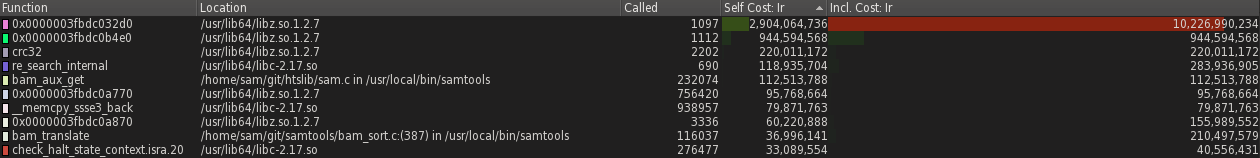
\includegraphics[width=1.0\textwidth]{callgrind_compressoutput_default}
    \caption[callgrind-default]{callgrind output following merge with default
    output compression}
    \label{fig:callgrind-default}
\end{figure}

\begin{figure}[htbp!]
    \centering
    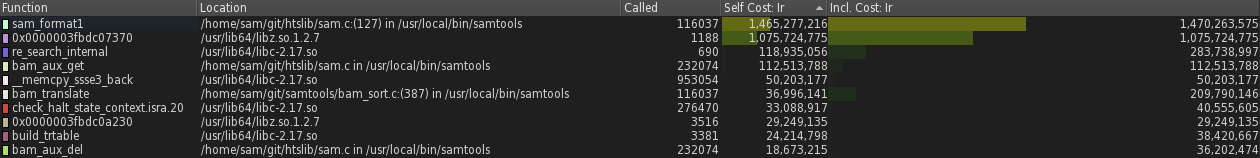
\includegraphics[width=1.0\textwidth]{callgrind_uncompressoutput}
    \caption[callgrind-uncompressed]{callgrind output following merge with
    uncompressed output}
    \label{fig:callgrind-uncompressed}
\end{figure}

% http://www.zlib.net/feldspar.html
Looking at a brief explanation of the deflate algorithm, it seems reasonable to
conclude the computational cost is rather asymmetric between compressing and
uncompressing - in that the effort is locating blocks to compress and in
comparison uncompressing is a reversible function on the known blocks.

Indeed, samtools merge specifies a -u option for uncompressed output and the
callgrind output (second image) indicates significantly less calls to zlib
functionality.

It remains to be seen whether this option will cut down the time needed for the
large merge job, perhaps this is merely a red herring and we’re yet to discover
the true speed trouble. In the meantime let’s see if sending this job to the
farm will work.


\subsubsection{The Red Herring}

% http://www.cs.utah.edu/dept/old/texinfo/as/gprof.html
... might be interesting to use gprof which is more
geared towards finding functions that spend all your execution time as opposed
to callgrind which I believe counts CPU instructions.

% http://paste.chippy.ch/woj.md
% https://github.com/samtools/htslib/blob/develop/sam.c#L1031
After re-compiling htslib and samtools with the -pg flag to enable such
profiling and executing the same previous merge command on the modest test set,
the output as parsed by gprof seems to indicate that the trouble lies with
bam\_aux\_get in htslib, with almost 50\% of the execution time being spent in
this particular function.

\begin{minted}[mathescape,
            %linenos,
            numbersep=5pt,
            %gobble=4,
            frame=lines,
            framesep=2mm]{c++}
    uint8_t *bam_aux_get(const bam1_t *b, const char tag[2])
    {
        uint8_t *s;
        int y = tag[0]<<8 | tag[1];
        s = bam_get_aux(b);
        while (s < b->data + b->l_data) {
            int x = (int)s[0]<<8 | s[1];
            s += 2;
            if (x == y) return s;
            s = skip_aux(s);
        }
        return 0;
    }
\end{minted}


% http://samtools.github.io/hts-specs/SAMv1.pdf
At a glance it seems that bam\_aux\_get receives a pointer to a BAM record and a
“tag”, an array of two characters representing an optional field as defined in
Section 1.5 of the SAM file spec.

The function then appears to fetch all these auxiliary tags and iterates over
each, comparing a transformation of that tag (x) to a pre-computed
transformation on the input tag (y).

% https://github.com/samtools/samtools/blob/2917ccdf34cd81b1327532b2db6e522fe871f054/bam_sort.c#L469
% https://github.com/samtools/samtools/blob/2917ccdf34cd81b1327532b2db6e522fe871f054/bam_sort.c#L484
% https://github.com/samtools/samtools/blob/2917ccdf34cd81b1327532b2db6e522fe871f054/bam_sort.c#L697
This would of course be inherently slow for files with many such tags;
especially given that the function is called twice for potentially each line in
a BAM file.


\subsubsection{The Plot Thickens}

% https://github.com/samtools/samtools/blob/2917ccdf34cd81b1327532b2db6e522fe871f054/bam_sort.c#L207
...as we increase the number of input files, the time taken to
read them in becomes non-linearly slower. Currently my money is on the seemingly
inefficient trans\_tbl\_init that appears to be called for each file, with the
current table of all previous files as an input.


\subsection{bcftools call}

...Unfortunately during the initial testing run of this step with all the
Goldilocks regions it was discovered that the output only included the standard
header information and not a single line for the variants themselves.
%\citep{biostar:bcftools} https://www.biostars.org/p/96425/

% http://samtools.github.io/bcftools/bcftools.html#call masked ref
...is because the piled up file was not generated with a corresponding reference
DNA sequence and so the REF (reference) column is set to N (an ambiguity code
which translates to ‘any base’).  bcftools call does have an -M flag to prevent
ignoring rows where the REF base is N (apparently called a "masked reference")
however this is currently causing a segmentation fault.  Having recompiled
htslib, samtools and bcftools I am now able to run bcftools call on my local
machine on some test data. I guess I’ll need to have someone recompile the
source for me on the cluster I’m using....




%%%%%%%%%%%%%%%%%%%%%%%%%%%%%%%%%%%%%%%%%%%%%%%%%%%%%%%%%%%%%%%%%%%%%%%%%%%%%%%
\chapter{Current Status}

